\vspace{1cm}
\section{Retrouver la loi}
\vspace{.2cm}

\noindent
À l’aide de 100 antennes GPS, en des points différents du globe\footnote{Éventuellement dans des environnements fortement métalliques ou partiellement enterrés}, le nombre de satellites visibles a été
compté :

\begin{center}
    \begin{tabular}{| c | c | c | c | c | c | c | c | c | c |}
        \hline
        Nombre de satellites & 1 & 2 & 3 & 4 & 5 & 6 & 7 & 8 & 9  \\ \hline
        Nombre d’observations & 6 & 15 & 9 & 25 & 17 & 10 & 8 & 7 & 3 \\ \hline
    \end{tabular}
\end{center}


%%%%%
\vspace{.5cm}
\begin{itemize}[label={},itemindent=-2em,leftmargin=2em]
    \item \textbf{Question~1~:} Estimer la moyenne et la variance de l’échantillon. Indication: on utilisera les opéra-
    teurs terme à terme python: \textit{**} et \textit{*}?
\end{itemize}
\vspace{.2cm}

\noindent
Formules utilisées~:

\begin{figure}[!h]
    \centering
    \begin{minipage}{.48\linewidth}
        \begin{equation}
            \overline{x}_{n} = \frac{\sum{(n_{i}.x_{i})}}{n}
        \end{equation}
    \end{minipage}\hfill\vline
    \begin{minipage}{.48\linewidth}
        \begin{equation}
            S^{2}_{n-1} = \frac{1}{n-1} \sum^{k}_{k=1}{n_{k}.(x_{k}-\overline{x}_{n})^{2}}
        \end{equation}
    \end{minipage}
\end{figure}



\begin{lstlisting}[style=myPython, caption=Code Python question 1, frame=lines]
obs = np.array([6, 15, 9, 25, 17, 10, 8, 7, 3])
sat = np.array([1, 2, 3, 4, 5, 6, 7, 8, 9])

nObs = 0
nSat = 0
for i in range(len(obs)):
    nObs += obs[i]
    nSat += sat[i]

num_mean = 0
for i in range(len(obs)):
    num_mean += obs[i]*sat[i]
mean = num_mean / nObs

num_var = 0
for i in range(len(obs)):
    num_var += (sat[i]-mean)**2
var = num_var/(len(sat)-1)

print("Question 1:")
print(" Moyenne =", mean)
print(' Variance =', var, end="\n\n")    
\end{lstlisting}

\begin{lstlisting}[style=myLog, caption=Résultat du code, frame=lines]
Question 1:
    Moyenne = 4.47
    Variance = 7.816012499999999
\end{lstlisting}

%%%%%
\vspace{.5cm}
\begin{itemize}[label={},itemindent=-2em,leftmargin=2em]
    \item \textbf{Question~2~:} Approcher la loi sous-jacente à l’aide d’une loi de Poisson de paramètre $\lambda = 4.47$. Déter-
    miner les effectifs théoriques pour 0 à 16 satellites. Indication: on utilisera la fonction \textit{poisson.pmf}.
\end{itemize}
\vspace{.2cm}

Grâce au code python ci-dessous, nous avons obtenus les effectifs théoriques suivants pour les satellites visibles de 0 à 16~:

\vspace{.1cm}

\begin{figure}[!h]
    \centering
    \begin{minipage}{.42\linewidth}
        \begin{center}
            \begin{tabular}{| c | c | c | c |}
                \hline
                \multicolumn{2}{|c|}{\textbf{Donnés}} & \multicolumn{2}{|c|}{\textbf{Estimés}} \\ \hline
                \textbf{Nb sat} & \textbf{Nb d'obs} & \textbf{Proba} & \textbf{eff th} \\ \hline\hline
                0 & N.C & 0.011 & 1.145 \\ \hline\hline
                1 & 6 & 0.051 & 5.117 \\ 
                2 & 15 & 0.114 & 11.436 \\ 
                3 & 9 & 0.17 & 17.04 \\ 
                4 & 25 & 0.19 & 19.042 \\
                5 & 17 & 0.17 & 17.024 \\ 
                6 & 10 & 0.127 & 12.683 \\ 
                7 & 8 & 0.081 & 8.099 \\ 
                8 & 7 & 0.045 & 4.525 \\ 
                9 & 3 & 0.022 & 2.248 \\ \hline\hline
                10 & N.C & 0.01 & 1.005 \\ 
                11 & N.C & 0.004 & 0.408 \\ 
                12 & N.C & 0.002 & 0.152 \\ 
                13 & N.C & 0.001 & 0.052 \\ 
                14 & N.C & 0.0 & 0.017 \\ 
                15 & N.C & 0.0 & 0.005 \\ 
                16 & N.C & 0.0 & 0.001 \\ \hline
            \end{tabular}
        \end{center}
    \end{minipage}\hfill
    \begin{minipage}{.54\linewidth}
        \begin{center}
            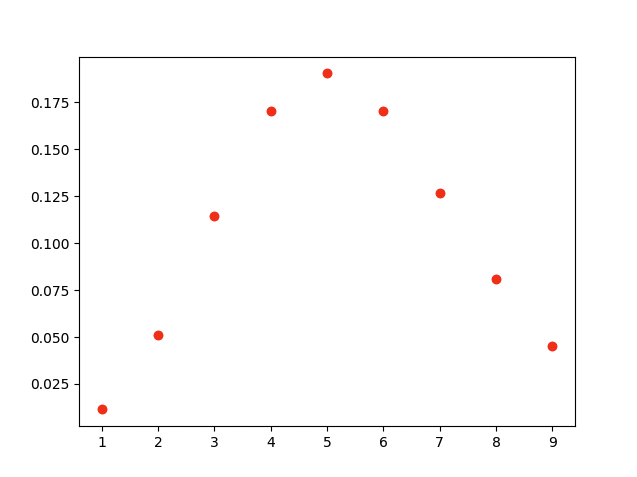
\includegraphics[width=1\textwidth]{img/figure1.png}
            \caption{\label{fig:figure1}Loi sous-jacente approcher par une loi de Poisson pour 1 à 9~satellites}

            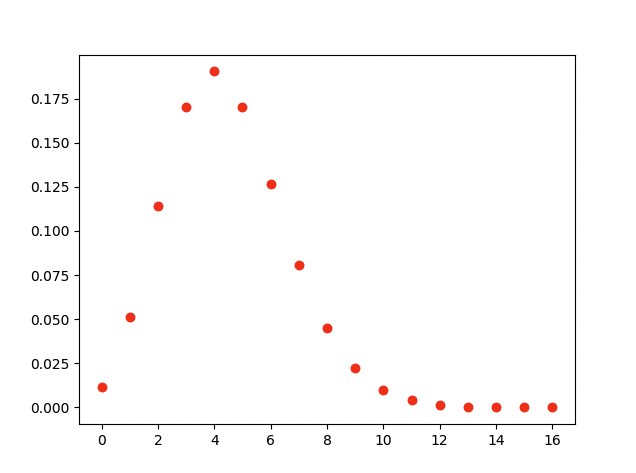
\includegraphics[width=1\textwidth]{img/figure2.png}
            \caption{\label{fig:figure1}Loi sous-jacente approcher par une loi de Poisson pour 0 à 16~satellites}
        \end{center}
    \end{minipage}
\end{figure}


\vspace{.1cm}

\begin{lstlisting}[style=myPython, caption=Code Python question 2, frame=lines]
Lambda = 4.47
poisson_array = np.zeros((17,))
effectifs_th = np.zeros((17,))
print("Question 2:")
print("nb Sat |  nb Obs  |  Proba  |   eff th")
print("=========================================")
poisson_array[0] = stats.poisson.pmf(0, Lambda)
effectifs_th[0] = nObs * poisson_array[0]
print("  ", 0, "  |  ", "N.C", "  |\t", round(poisson_array[0], 3), "\t|\t", round(effectifs_th[0], 3))
print("-----------------------------------------")

for i in range(1, len(sat)+1):
    poisson_array[i] = stats.poisson.pmf(sat[i-1], Lambda)
    effectifs_th[i] = nObs * poisson_array[i]

    print("  ", sat[i-1], "  |   ", round(obs[i-1], 2), "\t |\t", round(poisson_array[i], 3), "\t|\t", round(effectifs_th[i], 3))

print("-----------------------------------------")

plt.plot(sat, poisson_array[:9], 'ro')
plt.show()

for i in range(10, 17):
    poisson_array[i] = stats.poisson.pmf(i, Lambda)
    effectifs_th[i] = nObs * poisson_array[i]

    print(" ", i, "  |  ", "N.C", "  |\t", round(poisson_array[i], 3), "\t|\t", round(effectifs_th[i], 3))

print("\n\n")

nSat16 = np.arange(0, 17, 1)
plt.plot(nSat16, poisson_array, 'ro')
plt.show()
\end{lstlisting}

\begin{lstlisting}[style=myLog, caption=Résultat du code, frame=lines]
Question 2:
    nb Sat |  nb Obs  |  Proba  |   eff th
    =========================================
       0   |   N.C   |	 0.011 	|	 1.145
    -----------------------------------------
       1   |    6 	 |	 0.051 	|	 5.117
       2   |    15 	 |	 0.114 	|	 11.436
       3   |    9 	 |	 0.17 	|	 17.04
       4   |    25 	 |	 0.19 	|	 19.042
       5   |    17 	 |	 0.17 	|	 17.024
       6   |    10 	 |	 0.127 	|	 12.683
       7   |    8 	 |	 0.081 	|	 8.099
       8   |    7 	 |	 0.045 	|	 4.525
       9   |    3 	 |	 0.022 	|	 2.248
    -----------------------------------------
      10   |   N.C   |	 0.01 	|	 1.005
      11   |   N.C   |	 0.004 	|	 0.408
      12   |   N.C   |	 0.002 	|	 0.152
      13   |   N.C   |	 0.001 	|	 0.052
      14   |   N.C   |	 0.0 	  |	 0.017
      15   |   N.C   |	 0.0 	  |	 0.005
      16   |   N.C   |	 0.0 	  |	 0.001
\end{lstlisting}

%%%%%
\clearpage
\begin{itemize}[label={},itemindent=-2em,leftmargin=2em]
    \item \textbf{Question~3~:} Peut-on, à un seuil de $95\%$, considérer que l’échantillon a été produit par cette loi de
    Poisson ? \\
    Indication: Attention aux hypothèses, on utilisera les fonctions \textit{np.sum} et \textit{chi2.ppf}, les opérateurs
    terme à terme \textit{**} et \textit{/}, ainsi que l’extraction d’une tranche d’un vecteur par \textit{tab[i:j]}
\end{itemize}
\vspace{.2cm}

Dans un premier temps, on constate que les $n.p_{i}$ ne sont pas tous supérieurs à 1. \\
Les extrémités ont des effectifs plus faibles, on va donc les sommer jusqu'à dépasser 5, tout en réduisant 
de 1 la valeur de $k$ à chaque somme~:

\vspace{.1cm}

\begin{lstlisting}[style=myPython, caption=$n.p_{i} < 5$, frame=lines]
i = 0
while (effectifs_th[i] < 5):
    effectifs_th[i+1] += effectifs_th[i]
    effectifs_th[i] = 0
    i += 1

i = len(effectifs_th)-1
while (effectifs_th[i] < 5):
    effectifs_th[i-1] += effectifs_th[i]
    effectifs_th[i] = 0
    i -= 1

effectifs_th = np.delete(effectifs_th, np.where(effectifs_th == 0))
print("Les effectifs théorique après modification dû aux n.pi<5 :", effectifs_th)
\end{lstlisting}

\begin{lstlisting}[style=myLog, caption=Résultat du code, frame=lines]
Les effectifs théorique après modification dû aux n.pi<5 : 
[ 6.26168177 11.43638366 17.04021166 19.04243653 17.02393826 12.682834 8.09889543  8.41313506 ]
\end{lstlisting}

\vspace{.1cm}

\noindent
Maintenant que le test est conforme, on peut débuter les hypothèses et les calculs~:\\


\begin{enumerate}
    \item \textbf{Grandeur d'intérêt~:} La distribution du nombre de satellites visibles par rapport aux nombres de points d'observation.
    \vspace{.1cm}
   \item \textbf{Hypothèse nulle, $H0$~:} La distribution du nombre de satellites par rapport aux nombres de points d'observation a été produite par cette loi de poisson.
    \vspace{.1cm}
   \item \textbf{Hypothèse alternative, $H1$~:} La distribution du nombre de satellites par rapport aux nombres de points d'observation n'a pas été produite par cette loi de poisson.
    \vspace{.1cm}
   \item \textbf{Niveau de confiance~:} $95\%$
    \vspace{.1cm}
   \item \textbf{Test statistique~:} $\chi^{2}_{0} = \sum^{k}_{i=1} \frac{(n_{i} - np_{i})^{2}}{np_{i}}$ estimée par $\chi^{2}_{Obs}$ à partir de l'échantillon
    \vspace{.1cm}
   \item \textbf{Rejet de $H0$ si~:}
        \begin{itemize}
            \item Région critique: $\chi^{2}_{Obs} > \chi^{2}_{k-p-1, \alpha}$
            \item p-valeur: $p-valeur < 0.05$
        \end{itemize}

    \vspace{.1cm}
    \item \textbf{Calculs~:}
    \begin{itemize}
        \item Formules utilisées:
            \begin{figure}[!h]
                \centering
                \begin{minipage}{.48\linewidth}
                    \begin{equation}
                        \chi^{2}_{Obs} = \sum^{k}_{i=1} \frac{(n_{i} - np_{i})^{2}}{np_{i}}
                    \end{equation}
                \end{minipage}\hfill\vline
                \begin{minipage}{.48\linewidth}
                    \begin{equation}
                        \chi^{2}_{k-p-1, \alpha} = F^{-1}_{\chi^{2}_{k-p-1}}(\alpha)
                    \end{equation}
                \end{minipage}
            \end{figure}

            \begin{equation}
                \textit{p-valeur} = 1 - F_{\chi^{2}_{k-p-1}}(\chi^{2}_{Obs})
            \end{equation}
        
        \item Paramètres à prendre en compte~: \\
            \hspace*{1cm}$p \to$ Nombre de paramètres estimés~: 3 (moyenne, effectif théorique, loi poisson) \\
            \hspace*{1cm}$k \to$ Nombre de classe~: $\neq 16$, la condition~$n.p_{i} > 5$ n'était pas respectée

        
    \end{itemize}
        \vspace{.2cm}

\begin{lstlisting}[style=myPython, caption=Code Python question 3, frame=lines]
k = len(effectifs_th)
p = 3 # la moyenne, l'effectif th et loi poisson
ic = 95
alpha = 1 - ic / 100
chi2 = stats.chi2.ppf(1-alpha, k-p-1)
chi2_Obs = 0

for i in range(k):
    chi2_Obs += ((obs[i]-effectifs_th[i])**2)/(effectifs_th[i])

p_valeur = 1 - stats.chi2.cdf(chi2_Obs, k-p-1)

print("Question 3:")
print(" Chi2:", chi2)
print(" Chi2 Obs:", chi2_Obs)
print(" p-valeur:", p_valeur)
\end{lstlisting}

\begin{lstlisting}[style=myLog, caption=Résultat du code, frame=lines]
Question 3:
    Chi2: 9.487729036781154
    Chi2 Obs: 7.585020824300105
    p-valeur: 0.10801814641379404
\end{lstlisting}


    \item \textbf{Décision~:}
        \begin{figure}[!h]
            \centering
            \begin{minipage}{.48\linewidth}
                \begin{center}
                    \begin{tabular}{| c | c |}
                        \hline
                        \multicolumn{2}{| c |}{\textbf{Critéres de rejet de H0}} \\
                        pour $\alpha$ fixé & avec \textit{p-valeur} \\ \hline
                        $\chi^{2}_{Obs} > \chi^{2}_{k-p-1, \alpha}$ & $ \textit{p-valeur} < 0.05 $\\ \hline
                    \end{tabular}
                \end{center}
            \end{minipage}\hfill\vline
            \begin{minipage}{.48\linewidth}
                \begin{equation*}
                    \left .
                    \begin{aligned}
                        \chi^{2}_{Obs} = 7.585 \\
                        \chi^{2}_{k-p-1, \alpha} = 9.487\\
                        \textit{p-valeur} = 0.1
                    \end{aligned} \qquad
                    \right\} \qquad
                    \begin{aligned} 
                        \chi^{2}_{Obs} < \chi^{2}_{k-p-1, \alpha}\\
                        \textit{p-valeur} > 0.05
                    \end{aligned}
                \end{equation*}
            \end{minipage}
        \end{figure}

        Les résultats du test statistique montrent que \textit{H0} ne peut être rejeté puisqu'aucune des conditions n'est validée. \\
        La distribution du nombre de satellites par rapport aux nombres de points d'observations a été produite par cette loi de poisson.
\end{enumerate}


